% !TeX spellcheck = en_US

\chapter{Concept Description}

	uFixit is a platform on which users can get repair manuals. It does not matter from which manufacturer it comes, it works with all products of any brand. There is only one minor constraint: The part has to be fixable.
	
	\begin{figure}[H]
		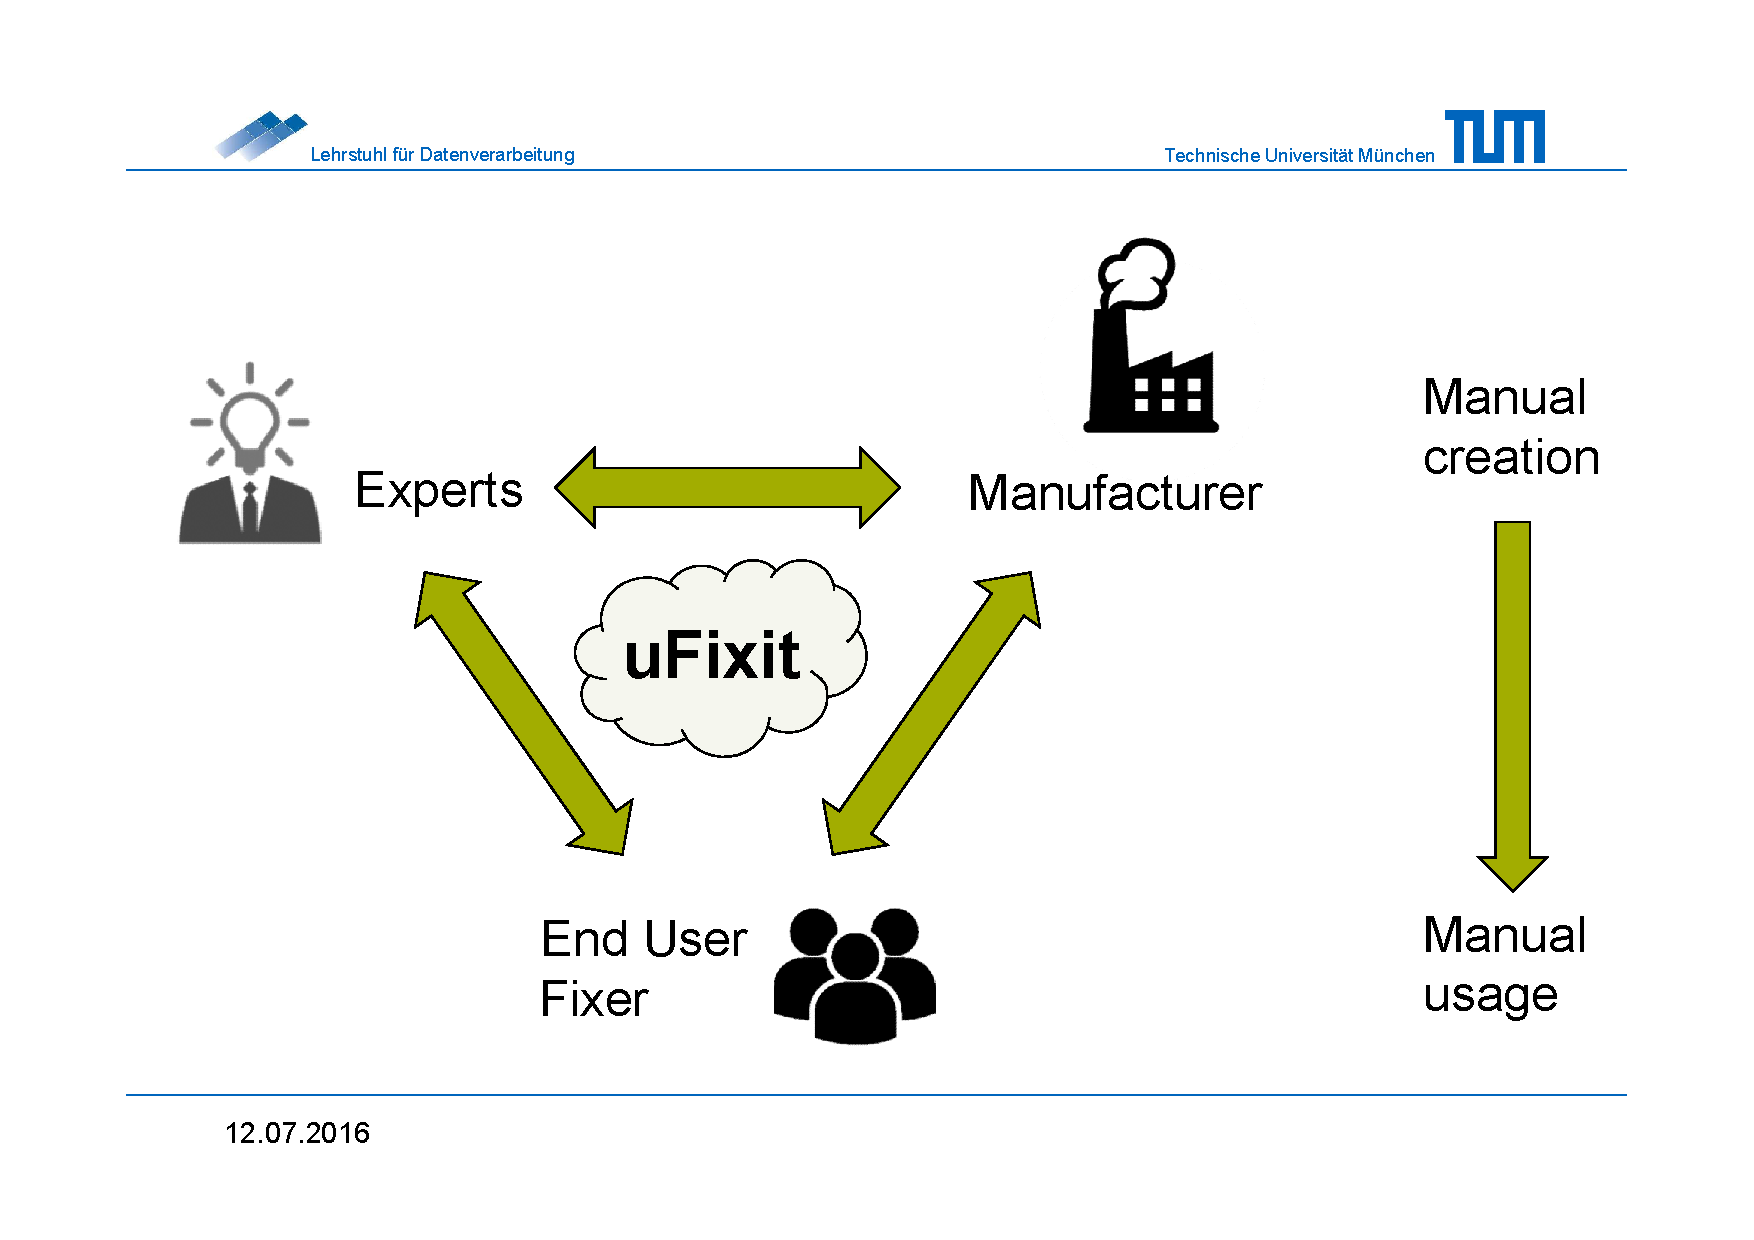
\includegraphics[width=\textwidth, trim=0cm 3cm 0cm 4cm, clip]{../images/involved-parties.pdf}
		\centering
		\caption{Parties involved in the uFixit environment}
		\label{fig:involved-parties}
	\end{figure}

	As one can see in \autoref{fig:involved-parties}, \textbf{Experts} and \textbf{Manufacturers} create the manuals, whereas \textbf{Fixers} use them to repair items. An Expert is a person that has the same equipment as an end user, but uses it to create manuals. He will not have special training or software to do so. Manufacturers on the other side have detailed information and models of their products and therefore can develop high quality instruction steps with animations and extensive highlighting.
	
	After describing how the instructions inside a manual looks like, we discuss how uFixit helps experts as well as manufacturers in creating the best possible manuals for the end user. For the conclusion of this chapter we have a look at how the experts are motivated to create content for our platform.


	\section{Instructions format}
	\label{sec:instr-format}
	
		Every manual is separated into several individual steps. The first step is always the diagnosis because to do the repair itself, we do need to know what is broken. While holding the defective part into the FOV of the camera, uFixit will try to match it to an internal database. If this succeeds, the next step is to get the right manual and suitable tools.
		
		
		After the preparation phase, the actual repair process begins. In each step, the user will be asked to perform a specific task. Subsequently the manual moves to the next step. This is executed in the following ways:
		
		\begin{itemize}
			\itemsep0em
			\item The AR device constantly watches the fixer while performing the task. With the help pf tracking algorithms, the application can detect when a step is finished and will automatically jump to the next one.
			\item Ideally the used device has a microphone built in. With that, the fixer simply can issue a voice command.
			\item Although it is more of a feature to jump to a specific step in the tutorial, forward and backward buttons are provided on screen for easy access.
		\end{itemize}
		
		\begin{figure}[H]
			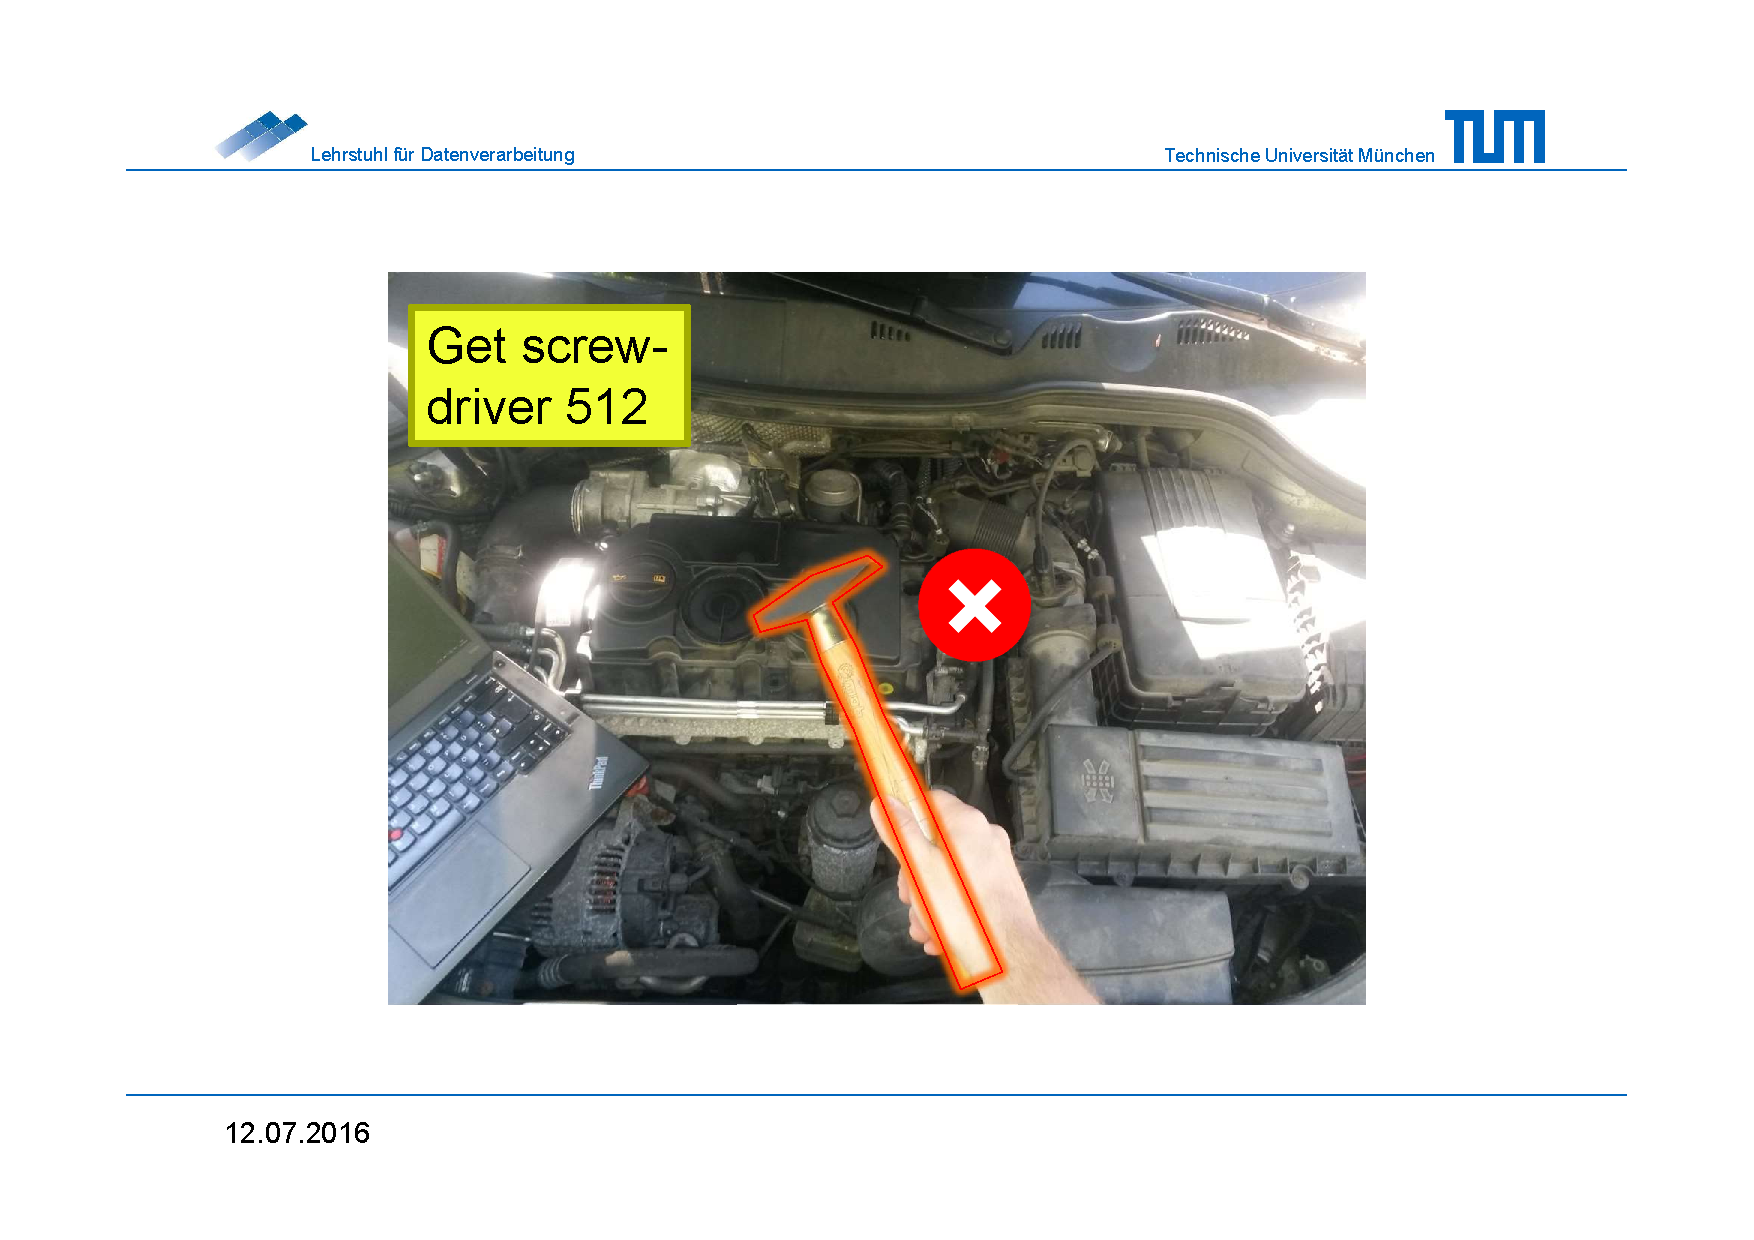
\includegraphics[width=\textwidth, trim=4cm 3cm 4cm 4cm, clip]{../images/instr-hammer.pdf}
			\centering
			\caption{Application is highlighting the wrong tool with a flashing read shadow}
			\label{fig:instr-hammer}
		\end{figure}
		
		\begin{figure}[H]
			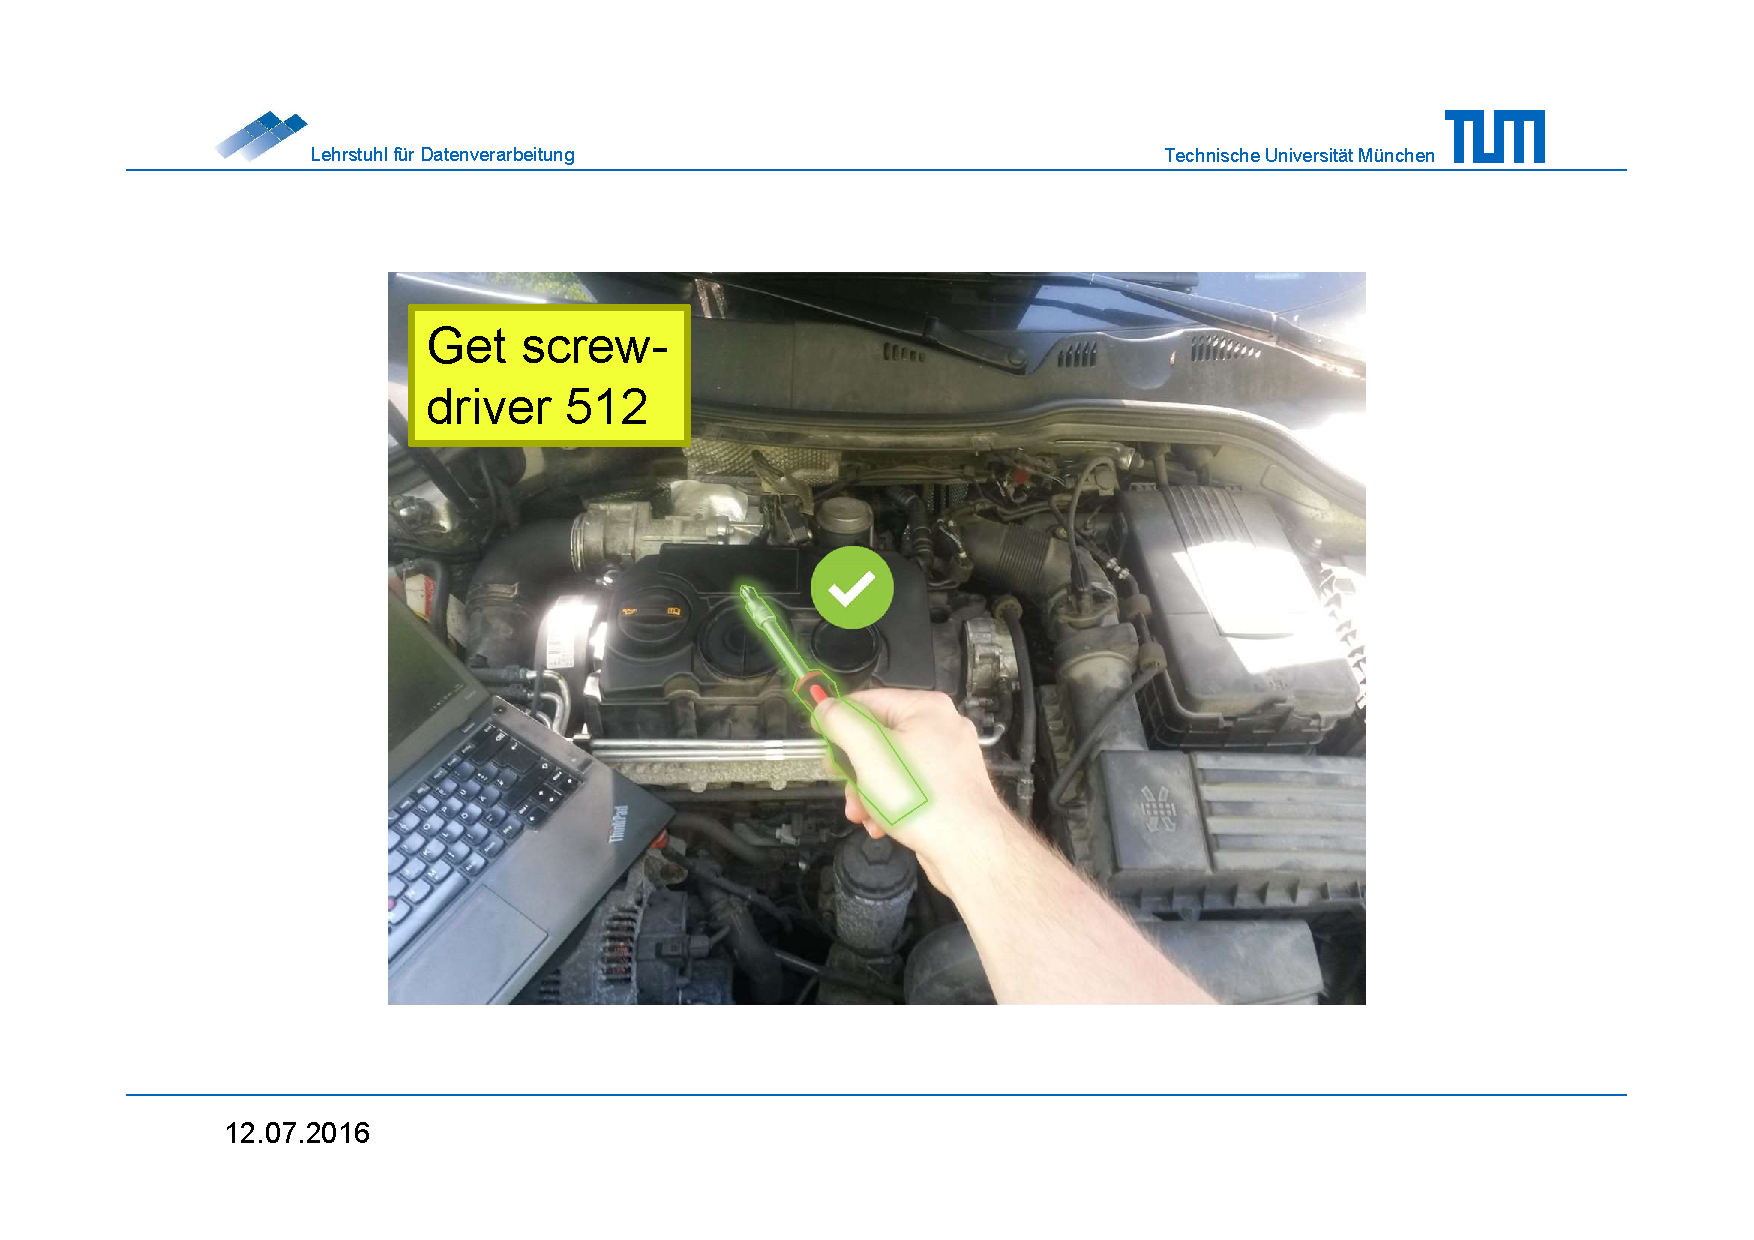
\includegraphics[width=\textwidth, trim=4cm 3cm 4cm 4cm, clip]{../images/instr-screwdriver.pdf}
			\centering
			\caption{When the Fixer picks up the right tool, the application will highlight it with a green shadow and after a short time transition to the next step}
			\label{fig:instr-screwdriver}
		\end{figure}
		
		\autoref{fig:instr-hammer} and \autoref{fig:instr-screwdriver} show how one instruction step looks like. The current task is shown in the top left corner - here: "Get screwdriver 512". When the user holds up a hammer, the AR device will register this tool and tell him that he is holding the wrong tool. After getting up the right tool, the manual will continue to the next step automatically.
		
	
	\section{Using existing AR hardware devices}
	
		One of the clous abouts uFixit is that the fixer can use almost every AR device on the market. It only has to fulfill a certain list of requirement that are described in chapter 3. Although users will get the most excellent experience with AR head mounted devices like the Microsoft HoloLens or the Meta 2 (\autoref{fig:meta2}), other devices like smartphones are also supported.
		
		\begin{figure}[H]
			\centering
			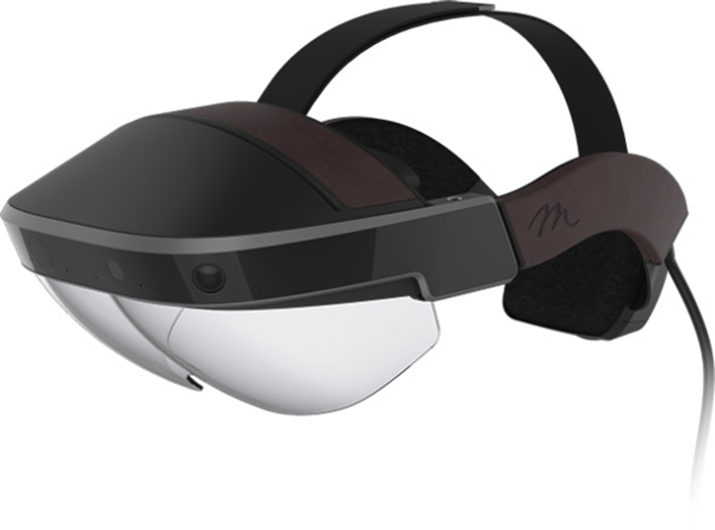
\includegraphics[width=0.5\linewidth]{../images/meta2.png}
			\caption{Meta 2 - Only one of the several devices uFixit will support}
			\label{fig:meta2}
		\end{figure}
		
		Although all kinds of smartphones are supported, there is special support for phones certifided for Google's Project Tango. This is basically an augmented reality platform definition for Android based phones and tables.
		
		\begin{figure}[H]
			\centering
			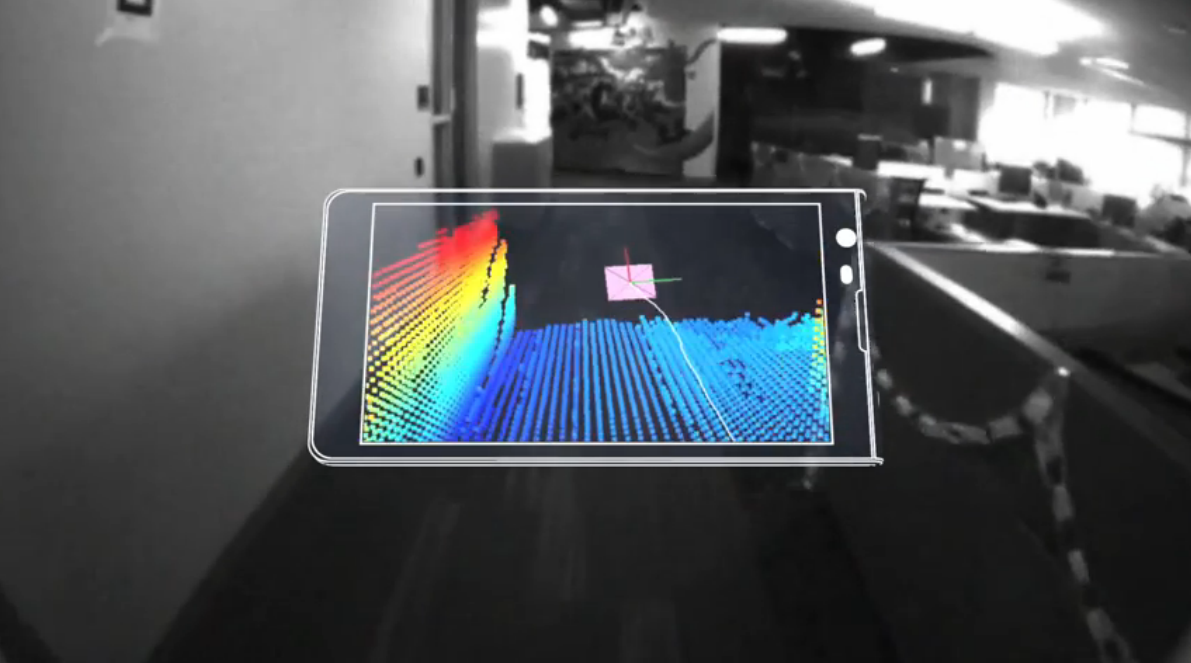
\includegraphics[width=0.7\linewidth]{../images/project-tango}
			\caption{Registration visualized using Project Tango by Google}
			\label{fig:project-tango}
		\end{figure}
		
		Of course if one does not have a suitable device, the manuals always can be watched using a webbrowser on a web portal as simple classical pages.
		
	
	\section{Software}
		
		Besides the application for the end user, the Fixer app, there are two additional software packages that are responsible for the content creation. They can be seen in \autoref{fig:software-overview}.
		
		\begin{figure}[H]
			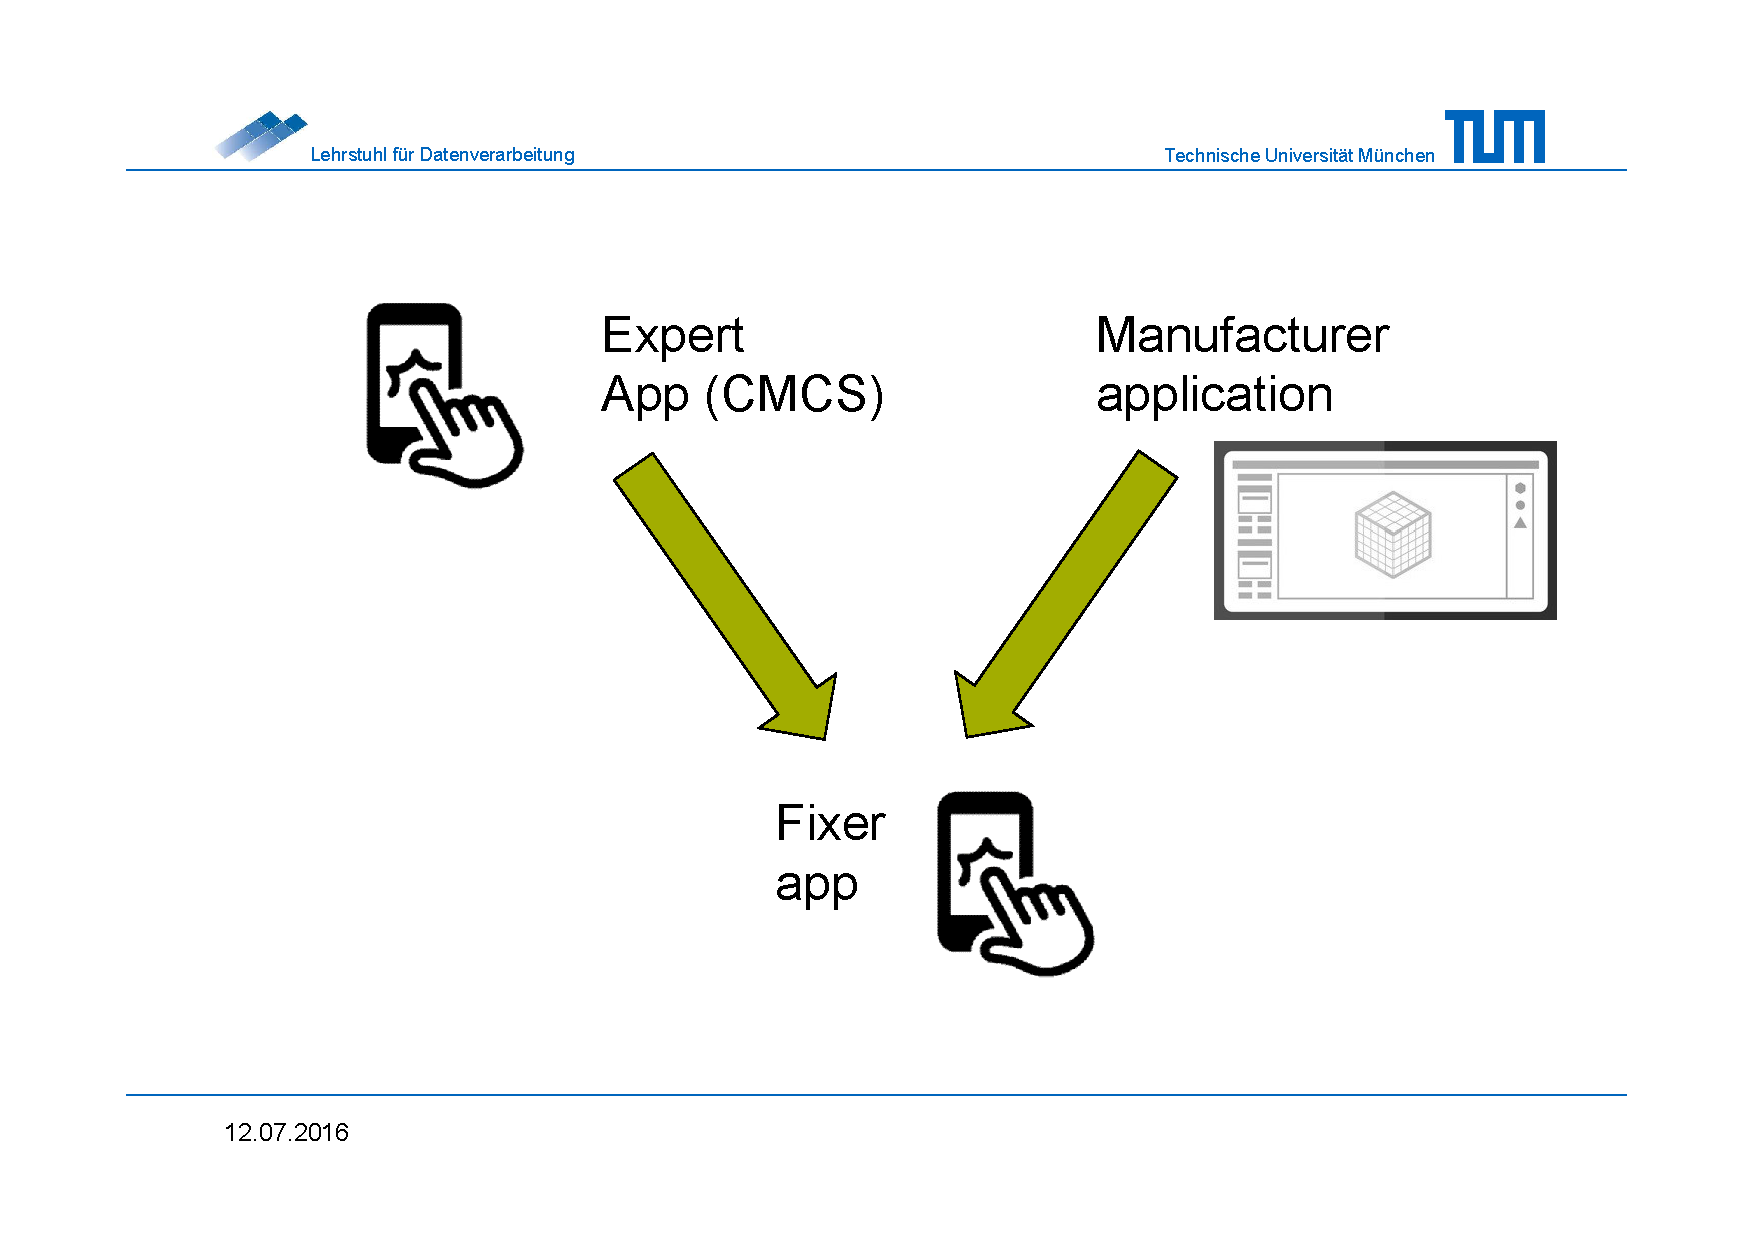
\includegraphics[width=\textwidth, trim=4cm 3cm 3cm 4cm, clip]{../images/software-overview.pdf}
			\centering
			\caption{uFixit applications Eco-system}
			\label{fig:software-overview}
		\end{figure}
		
		The Experts are creating their manuals with a simple, intuitive and fool proof app on the same AR devices the Fixer uses. It is called \textbf{Community Manual Creation Software} (CMCS). The main goal is to make creating manuals available for everybody.
		
		Manufacturers will receive plugins for the various 3D CAD programs to seamlessly integrate with their already existing environment. Naturally the exported steps can be as complex as the manual engineer likes. Especially the things that can not be done with the Community Manual Creation Software are the most interesting:
		
		\begin{itemize}
			\itemsep0em
			\item animations
			\item see through content
			\item user defined masking of obscuring parts
		\end{itemize}
		
		Since every single AR device is unique in its own way, the \textbf{Fixer app} will provided a intuitive workflow specific to the device it runs on. It will still follow these three steps:
		
		\begin{enumerate}
			\itemsep0em
			\item Diagnosis: Find out what product the user wants to repair and how it is broken.
			\item Preparation: Obtain tools and manuals for next step
			\item Actual repair as described in \eqref{sec:instr-format}
		\end{enumerate}
		
		
	\section{Experts Reward Program}
	
		uFixit relies heavily on the Fixers to get involved in the community and to start creating own manuals. This can solely be based on idealism. Believing this would work on the other hand is pretty naive. Our solution: Money!
		
		Many big software companies nowadays have something called bug bounty program. This means if a person finds a bug of a certain severity in the manufacturer’s product, he will get rewarded when reporting it. This is very convenient for the company considering they do not have to pay everyone that is searching for these flaws in the software.
		
		We want the same principle integrated into uFixit. Experts should be lured into a \textbf{manual bounty program} that will reward them every time a Fixer solves a problem using his tutorial. The money will come from the manufacturer who will benefit from only paying a small amount for high quality content rather to spend more for trained personal..
	
	\section{Feedback}
	
		To provide the user with highest quality manuals, there will be an opportunity to rate them with a review system. Online shopping nowadays would be unimaginable without reviews just because no one likes to buy untested products. Especially when the end user needs quick and good help, he is more willing to invest in a manual that has a 100\% rating instead of first trying the free one, with 75\% rating.

		\begin{figure}[H]
			\centering
			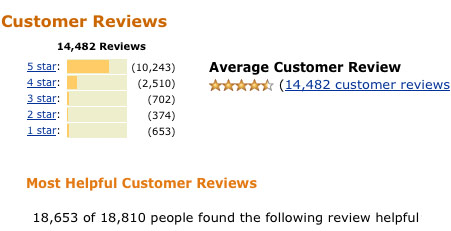
\includegraphics[width=0.7\linewidth]{../images/how-to-get-amazon-reviews-kindle.jpg}
			\caption{Example of product reviews on \url{amazon.com} with a overwhelming good average rating}
			\label{fig:amazon-reviews}
		\end{figure}
		
		\autoref{fig:amazon-reviews} is a screenshot from the \url{amazon.com} website. It shows a product review page with an overwhelming good average rating. Most of the users would now be convinced this is a great product and buy it without further research or thinking. the uFixit review system will be quite similar to this one because it will increase community involvement and building.
